\IfFileExists{stacks-project.cls}{%
\documentclass{stacks-project}
}{%
\documentclass{amsart}
}
\usepackage{amssymb}

% For dealing with references we use the comment environment
\usepackage{verbatim}
\usepackage{fancyvrb}
\usepackage{pmboxdraw}
\newenvironment{reference}{\comment}{\endcomment}
%\newenvironment{reference}{}{}
\newenvironment{slogan}{\comment}{\endcomment}
\newenvironment{history}{\comment}{\endcomment}

% For source figures retained as assets
\usepackage{graphicx}

% For commutative diagrams we use Xy-pic
\usepackage[all]{xy}

% We use 2cell for 2-commutative diagrams.
\xyoption{2cell}
\UseAllTwocells

% We use multicol for the list of chapters between chapters
\usepackage{multicol}

% This is generally recommended for better output
\usepackage{lmodern}
\usepackage[T1]{fontenc}
\usepackage{textalpha}

% For cross-file-references
% We prefer the snapshot tmp/xref/#2.aux,
% which latexmkrc replaces atomically, so
% that documents compiled simultaneously
% never read a half-written .aux file.
% The last argument keeps links to #2.pdf.
\usepackage{xr-hyper}
\newcommand{\maybeexternaldocument}[2]{%
  \IfFileExists{#2.aux}{%
    \externaldocument[#1]{#2}%
  }{%
    \PackageWarning{stack}{Missing #2.aux; external references with prefix #1 unavailable}%
  }%
}
\let\externaldocumentorig\externaldocument
\renewcommand{\externaldocument}[2][]{%
  \IfFileExists{tmp/xref/#2.aux}{%
    \externaldocumentorig[#1]{tmp/xref/#2}[#2.pdf]%
  }{%
  \IfFileExists{#2.aux}{%
    \externaldocumentorig[#1]{#2}%
  }{%
    \PackageWarning{stack}{Missing #2.aux; external references with prefix #1 unavailable}%
  }%
  }%
}

% Package for hypertext links:
\usepackage{hyperref}

% For any local file, say "hello.tex" you want to link to please
% use \externaldocument[hello-]{hello}
\externaldocument[introduction-]{introduction}
\externaldocument[conventions-]{conventions}
\externaldocument[sets-]{sets}
\externaldocument[categories-]{categories}
\externaldocument[topology-]{topology}
\externaldocument[sheaves-]{sheaves}
\externaldocument[sites-]{sites}
\externaldocument[stacks-]{stacks}
\externaldocument[fields-]{fields}
\externaldocument[algebra-]{algebra}
\externaldocument[brauer-]{brauer}
\externaldocument[homology-]{homology}
\externaldocument[derived-]{derived}
\externaldocument[simplicial-]{simplicial}
\externaldocument[more-algebra-]{more-algebra}
\externaldocument[smoothing-]{smoothing}
\externaldocument[modules-]{modules}
\externaldocument[sites-modules-]{sites-modules}
\externaldocument[injectives-]{injectives}
\externaldocument[cohomology-]{cohomology}
\externaldocument[sites-cohomology-]{sites-cohomology}
\externaldocument[dga-]{dga}
\externaldocument[dpa-]{dpa}
\externaldocument[sdga-]{sdga}
\externaldocument[hypercovering-]{hypercovering}
\externaldocument[schemes-]{schemes}
\externaldocument[constructions-]{constructions}
\externaldocument[properties-]{properties}
\externaldocument[morphisms-]{morphisms}
\externaldocument[coherent-]{coherent}
\externaldocument[divisors-]{divisors}
\externaldocument[limits-]{limits}
\externaldocument[varieties-]{varieties}
\externaldocument[topologies-]{topologies}
\externaldocument[descent-]{descent}
\externaldocument[perfect-]{perfect}
\externaldocument[more-morphisms-]{more-morphisms}
\externaldocument[flat-]{flat}
\externaldocument[groupoids-]{groupoids}
\externaldocument[more-groupoids-]{more-groupoids}
\externaldocument[etale-]{etale}
\externaldocument[chow-]{chow}
\externaldocument[intersection-]{intersection}
\externaldocument[pic-]{pic}
\externaldocument[weil-]{weil}
\externaldocument[adequate-]{adequate}
\externaldocument[dualizing-]{dualizing}
\externaldocument[duality-]{duality}
\externaldocument[discriminant-]{discriminant}
\externaldocument[derham-]{derham}
\externaldocument[local-cohomology-]{local-cohomology}
\externaldocument[algebraization-]{algebraization}
\externaldocument[curves-]{curves}
\externaldocument[resolve-]{resolve}
\externaldocument[models-]{models}
\externaldocument[functors-]{functors}
\externaldocument[equiv-]{equiv}
\externaldocument[pione-]{pione}
\externaldocument[etale-cohomology-]{etale-cohomology}
\externaldocument[proetale-]{proetale}
\externaldocument[relative-cycles-]{relative-cycles}
\externaldocument[more-etale-]{more-etale}
\externaldocument[trace-]{trace}
\externaldocument[crystalline-]{crystalline}
\externaldocument[spaces-]{spaces}
\externaldocument[spaces-properties-]{spaces-properties}
\externaldocument[spaces-morphisms-]{spaces-morphisms}
\externaldocument[decent-spaces-]{decent-spaces}
\externaldocument[spaces-cohomology-]{spaces-cohomology}
\externaldocument[spaces-limits-]{spaces-limits}
\externaldocument[spaces-divisors-]{spaces-divisors}
\externaldocument[spaces-over-fields-]{spaces-over-fields}
\externaldocument[spaces-topologies-]{spaces-topologies}
\externaldocument[spaces-descent-]{spaces-descent}
\externaldocument[spaces-perfect-]{spaces-perfect}
\externaldocument[spaces-more-morphisms-]{spaces-more-morphisms}
\externaldocument[spaces-flat-]{spaces-flat}
\externaldocument[spaces-groupoids-]{spaces-groupoids}
\externaldocument[spaces-more-groupoids-]{spaces-more-groupoids}
\externaldocument[bootstrap-]{bootstrap}
\externaldocument[spaces-pushouts-]{spaces-pushouts}
\externaldocument[spaces-chow-]{spaces-chow}
\externaldocument[groupoids-quotients-]{groupoids-quotients}
\externaldocument[spaces-more-cohomology-]{spaces-more-cohomology}
\externaldocument[spaces-simplicial-]{spaces-simplicial}
\externaldocument[spaces-duality-]{spaces-duality}
\externaldocument[formal-spaces-]{formal-spaces}
\externaldocument[restricted-]{restricted}
\externaldocument[spaces-resolve-]{spaces-resolve}
\externaldocument[formal-defos-]{formal-defos}
\externaldocument[defos-]{defos}
\externaldocument[cotangent-]{cotangent}
\externaldocument[examples-defos-]{examples-defos}
\externaldocument[algebraic-]{algebraic}
\externaldocument[examples-stacks-]{examples-stacks}
\externaldocument[stacks-sheaves-]{stacks-sheaves}
\externaldocument[criteria-]{criteria}
\externaldocument[artin-]{artin}
\externaldocument[quot-]{quot}
\externaldocument[stacks-properties-]{stacks-properties}
\externaldocument[stacks-morphisms-]{stacks-morphisms}
\externaldocument[stacks-limits-]{stacks-limits}
\externaldocument[stacks-cohomology-]{stacks-cohomology}
\externaldocument[stacks-perfect-]{stacks-perfect}
\externaldocument[stacks-introduction-]{stacks-introduction}
\externaldocument[stacks-more-morphisms-]{stacks-more-morphisms}
\externaldocument[stacks-geometry-]{stacks-geometry}
\externaldocument[moduli-]{moduli}
\externaldocument[moduli-curves-]{moduli-curves}
\externaldocument[examples-]{examples}
\externaldocument[exercises-]{exercises}
\externaldocument[guide-]{guide}
\externaldocument[desirables-]{desirables}
\externaldocument[coding-]{coding}
\externaldocument[obsolete-]{obsolete}
\externaldocument[fdl-]{fdl}
\externaldocument[index-]{index}

% Heap Project documents
\externaldocument[k3-]{k3}
\externaldocument[torelli-]{torelli}
\externaldocument[linear-algebra-]{linear-algebra}
\externaldocument[groups-]{groups}
\externaldocument[complex-analysis-]{complex-analysis}
\externaldocument[functional-analysis-]{functional-analysis}
\externaldocument[categories-]{categories}
\externaldocument[commutative-algebra-]{commutative-algebra}
\externaldocument[ringed-spaces-]{ringed-spaces}
\externaldocument[homological-algebra-]{homological-algebra}
\externaldocument[lie-algebras-]{lie-algebras}
\externaldocument[representation-theory-]{representation-theory}
\externaldocument[smooth-manifolds-]{smooth-manifolds}
\externaldocument[differential-topology-]{differential-topology}
\externaldocument[algebraic-topology-]{algebraic-topology}
\externaldocument[differential-geometry-]{differential-geometry}
\externaldocument[algebraic-geometry-]{algebraic-geometry}
\externaldocument[symplectic-geometry-]{symplectic-geometry}
\externaldocument[complex-geometry-]{complex-geometry}
\externaldocument[hodge-theory-]{hodge-theory}
\externaldocument[%
variations-of-hodge-structures-]{%
variations-of-hodge-structures}
\externaldocument[%
homological-mirror-symmetry-]{%
homological-mirror-symmetry}
\maybeexternaldocument{deformations-}{deformations}
\externaldocument[vertex-algebras-]{vertex-algebras}
\externaldocument[springer-]{springer}
\externaldocument[infty-categories-]{infty-categories}
\externaldocument[seminars-differential-geometry-]{%
seminars-differential-geometry}
\externaldocument[seminars-complex-geometry-]{%
seminars-complex-geometry}
\externaldocument[seminars-algebraic-geometry-]{%
seminars-algebraic-geometry}
\externaldocument[seminars-analysis-pde-]{%
seminars-analysis-pde}
\externaldocument[surfaces-]{surfaces}
\externaldocument[birational-maps-commutative-algebra-]{birational-maps-commutative-algebra}
\externaldocument[cremona-transformations-]{cremona-transformations}
\externaldocument[derived-categories-of-sheaves-]{derived-categories-of-sheaves}
\externaldocument[geometric-invariant-theory-]{geometric-invariant-theory}
\externaldocument[geometric-stability-conditions-and-group-actions-]{geometric-stability-conditions-and-group-actions}
\externaldocument[moduli-spaces-of-sheaves-]{moduli-spaces-of-sheaves}
\externaldocument[bridgeland-stability-general-theory-]{bridgeland-stability-general-theory}
\externaldocument[hilbert-schemes-]{hilbert-schemes}
\externaldocument[noncommutative-abelian-surfaces-and-kummer-type-hyperkahler-varieties-]{noncommutative-abelian-surfaces-and-kummer-type-hyperkahler-varieties}
\externaldocument[mumford-tate-groups-in-hodge-theory-]{mumford-tate-groups-in-hodge-theory}
\externaldocument[hodge-birational-atoms-2026-]{hodge-birational-atoms-2026}
\externaldocument[xxii-egd-2026-]{%
xxii-egd-2026}
\externaldocument[pde-]{pde}
\externaldocument[probability-]{probability}

\externaldocument[linguistics-]{linguistics}

\externaldocument[%
16th-alga-meeting-2026-]{%
16th-alga-meeting-2026}

\externaldocument[%
iv-jornadas-lefschetz-2026-]{%
iv-jornadas-lefschetz-2026}

\externaldocument[reading-the-masters-]{%
reading-the-masters}

\externaldocument[real-analysis-]{%
real-analysis}

\externaldocument[optimal-transport-]{%
optimal-transport}

\externaldocument[history-]{history}

\externaldocument[seiberg-witten-]{seiberg-witten}

\externaldocument[history-philosophy-biology-]{history-philosophy-biology}

\externaldocument[classical-mechanics-]{classical-mechanics}
\externaldocument[electromagnetism-]{electromagnetism}
\externaldocument[waves-and-optics-]{waves-and-optics}
\externaldocument[wif-]{waves-in-fluids-iv}
\externaldocument[thermal-physics-]{thermal-physics}
\externaldocument[quantum-mechanics-]{quantum-mechanics}
\externaldocument[special-relativity-]{special-relativity}
\externaldocument[physics-]{physics}

\externaldocument[chemistry-]{chemistry}

\externaldocument[molecular-cell-biology-]{molecular-cell-biology}

\externaldocument[microbiology-]{microbiology}

\externaldocument[protistology-]{protistology}

\externaldocument[mycology-]{mycology}

\externaldocument[botany-]{botany}

\externaldocument[zoology-]{zoology}

\externaldocument[animal-histology-]{animal-histology}

\externaldocument[animal-physiology-]{animal-physiology}

\externaldocument[systematics-biogeography-]{systematics-biogeography}

\externaldocument[ecology-natural-resources-]{ecology-natural-resources}

\externaldocument[earth-sciences-]{earth-sciences}

\externaldocument[biostatistics-]{biostatistics}

\externaldocument[mathematical-systems-biology-]{mathematical-systems-biology}

\externaldocument[cimpa-el-salvador-2024-]{cimpa-el-salvador-2024}

\externaldocument[anthropology-]{anthropology}

\externaldocument[yang-mills-theory-]{yang-mills-theory}

\externaldocument[seminars-algebra-]{seminars-algebra}

\externaldocument[seminars-physics-]{seminars-physics}

\externaldocument[seminars-computing-]{seminars-computing}

\externaldocument[oktobermat-2026-]{oktobermat-2026}

\externaldocument[saet-2026-]{saet-2026}

\externaldocument[seminars-symplectic-geometry-]{seminars-symplectic-geometry}

\externaldocument[seminars-dynamics-]{seminars-dynamics}

\externaldocument[oktobermat-2024-]{oktobermat-2024}

\externaldocument[quantum-groups-]{quantum-groups}

\externaldocument[legal-2027-]{legal-2027}

\externaldocument[derived-categories-]{derived-categories}

% Theorem environments.
%
\theoremstyle{plain}
\newtheorem{theorem}[subsection]{Theorem}
\newtheorem{proposition}[subsection]{Proposition}
\newtheorem{lemma}[subsection]{Lemma}
\newtheorem{corollary}[subsection]{Corollary}

\theoremstyle{definition}
\newtheorem{definition}[subsection]{Definition}
\newtheorem{example}[subsection]{Example}
\newtheorem{exercise}[subsection]{Exercise}
\newtheorem{situation}[subsection]{Situation}

\theoremstyle{remark}
\newtheorem{remark}[subsection]{Remark}
\newtheorem{remarks}[subsection]{Remarks}

\numberwithin{equation}{subsection}

% Macros
%
\def\lim{\mathop{\mathrm{lim}}\nolimits}
\def\colim{\mathop{\mathrm{colim}}\nolimits}
\def\Spec{\mathop{\mathrm{Spec}}}
\def\Hom{\mathop{\mathrm{Hom}}\nolimits}
\def\Ext{\mathop{\mathrm{Ext}}\nolimits}
\def\SheafHom{\mathop{\mathcal{H}\!\mathit{om}}\nolimits}
\def\SheafExt{\mathop{\mathcal{E}\!\mathit{xt}}\nolimits}
\def\Sch{\mathit{Sch}}
\def\Mor{\mathop{\mathrm{Mor}}\nolimits}
\def\Ob{\mathop{\mathrm{Ob}}\nolimits}
\def\Sh{\mathop{\mathit{Sh}}\nolimits}
\def\NL{\mathop{N\!L}\nolimits}
\def\CH{\mathop{\mathrm{CH}}\nolimits}
\def\proetale{{pro\text{-}\acute{e}tale}}
\def\etale{{\acute{e}tale}}
\def\QCoh{\mathit{QCoh}}
\def\Ker{\mathop{\mathrm{Ker}}}
\def\Im{\mathop{\mathrm{Im}}}
\def\Coker{\mathop{\mathrm{Coker}}}
\def\Coim{\mathop{\mathrm{Coim}}}

% Boxtimes
%
\DeclareMathSymbol{\boxtimes}{\mathbin}{AMSa}{"02}

%
% Macros for moduli stacks/spaces
%
\def\QCohstack{\mathcal{QC}\!\mathit{oh}}
\def\Cohstack{\mathcal{C}\!\mathit{oh}}
\def\Spacesstack{\mathcal{S}\!\mathit{paces}}
\def\Quotfunctor{\mathrm{Quot}}
\def\Hilbfunctor{\mathrm{Hilb}}
\def\Curvesstack{\mathcal{C}\!\mathit{urves}}
\def\Polarizedstack{\mathcal{P}\!\mathit{olarized}}
\def\Complexesstack{\mathcal{C}\!\mathit{omplexes}}
% \Pic is the operator that assigns to X its picard group, usage \Pic(X)
% \Picardstack_{X/B} denotes the Picard stack of X over B
% \Picardfunctor_{X/B} denotes the Picard functor of X over B
\def\Pic{\mathop{\mathrm{Pic}}\nolimits}
\def\Picardstack{\mathcal{P}\!\mathit{ic}}
\def\Picardfunctor{\mathrm{Pic}}
\def\Deformationcategory{\mathcal{D}\!\mathit{ef}}


\begin{document}

\title{Tessellations of the plane}
\maketitle

\phantomsection
\label{section-phantom}

\tableofcontents

\section{Introduction}
\label{section-introduction}

\noindent
This chapter is an account in English of the
author's bachelor's thesis
\cite{gca-tesis-licenciatura}, written under
the supervision of Vinicio Antonio G\'omez
Guti\'errez. The thesis has two parts. The
first is an introduction to the theory of
tilings of the Euclidean plane, following the
first two chapters of
\cite{GrunbaumShephard1987}. The second goes
through the 17 symmetry groups of periodic
tilings, following
\cite{Martin1982}: for each group it
constructs a unit cell, finds generators, and
gives a presentation by generators and
relations. Further presentations of the 17
groups are tabulated in
\cite{CoxeterMoser1957}; see also
\cite{Schattschneider1978} for the notation
and for how to recognise the groups.

The thesis is mostly a visual text, and most
of its illustrations are built on the periodic
drawings of M. C. Escher. The diagrams of unit
cells reproduced below are taken from it.
Statements are quoted from the sources named
next to them and are not proved here.

\section{Tilings}
\label{section-tilings}

\begin{definition}
\label{definition-tiling}
A \emph{tiling} (or \emph{tessellation}) of
the plane is a countable collection
$\mathcal{T}=\{T_1,T_2,T_3,\ldots\}$ of closed
subsets of the Euclidean plane $E^2$, called
\emph{tiles}, such that
\begin{enumerate}
\item the union of the tiles is the whole
plane, and the interiors of the tiles are
pairwise disjoint,
\item the boundary of every tile is a simple
closed curve,
\item the intersection of two tiles is empty,
a single point, or a single arc,
\item every vertex has finite valence.
\end{enumerate}
The points that lie in three or more tiles are
the \emph{vertices}. They divide the
boundaries of the tiles into arcs, the
\emph{edges}. The \emph{valence} of a vertex
is the number of edges that meet at it.
\end{definition}

\noindent
Condition (2) excludes unbounded tiles and
tiles with holes. Condition (3) excludes two
tiles that touch along two separate arcs.
Condition (4) excludes infinitely many tiles,
smaller and smaller, around one point. An edge
joins two vertices, and at least three edges
and three tiles meet at every vertex.

\begin{definition}
\label{definition-symmetry}
An \emph{isometry} is a map
$\sigma:E^2\to E^2$ that preserves distances.
A \emph{symmetry} of a figure $F\subset E^2$
is an isometry $\sigma$ with $\sigma(F)=F$.
A \emph{symmetry} of a tiling $\mathcal{T}$ is
an isometry that sends every tile onto a
tile. The symmetries of $\mathcal{T}$ form a
group under composition, the
\emph{symmetry group} $S(\mathcal{T})$.
\end{definition}

\noindent
Every isometry of the plane is of exactly one
of four kinds, besides the identity: a
rotation about a point, a translation, a
reflection in a line, or a glide reflection,
which is a reflection in a line followed by a
translation parallel to that line
\cite{GrunbaumShephard1987}.

The group $S(\mathcal{T})$ acts on the set of
tiles, on the set of edges and on the set of
vertices. The orbits are called
\emph{transitivity classes}.

\begin{definition}
\label{definition-isohedral}
A tiling is
\begin{enumerate}
\item \emph{monohedral} if all tiles are
congruent, and \emph{$k$-hedral} if there are
$k$ tiles such that every tile is congruent to
exactly one of them,
\item \emph{isohedral} if its symmetry group
is transitive on tiles, and
\emph{$k$-isohedral} if there are $k$
transitivity classes of tiles,
\item \emph{isogonal} if its symmetry group is
transitive on vertices,
\item \emph{isotoxal} if its symmetry group is
transitive on edges,
\item \emph{regular} if its symmetry group is
transitive on flags, where a \emph{flag} is a
triple $(V,E,T)$ of a vertex $V$, an edge $E$
containing $V$ and a tile $T$ containing $E$.
\end{enumerate}
\end{definition}

\noindent
An isohedral tiling is monohedral. The
converse fails: two tiles may be congruent by
an isometry that is not a symmetry of the
tiling.

\section{Tilings by regular polygons and
their duals}
\label{section-regular-polygons}

\noindent
A tiling by polygons is \emph{edge-to-edge} if
every side of every polygon is an edge of the
tiling. All statements in this section are
from \cite[Chapter 2]{GrunbaumShephard1987}.

\begin{theorem}
\label{theorem-regular-tilings}
Up to similarity there are exactly three
regular tilings of the plane: by equilateral
triangles, by squares and by regular
hexagons. They are also the only edge-to-edge
monohedral tilings by regular polygons.
\end{theorem}

\noindent
Now allow regular polygons of several kinds.
Suppose that $r$ regular polygons with
$n_1,\ldots,n_r$ sides fit around a vertex.
The interior angle of a regular $n$-gon is
$(n-2)\pi/n$, so
$$
\frac{n_1-2}{n_1}+\frac{n_2-2}{n_2}+\cdots
+\frac{n_r-2}{n_r}=2.
$$
This equation has 17 solutions in integers
$n_i\geq3$. For four of them the polygons can
be arranged around the vertex in two different
cyclic orders, so there are 21 possible
\emph{vertex types}, written
$(n_1.n_2.\,\cdots.n_r)$ with exponents for
repetitions, as in $(3^4.6)$.

\begin{theorem}
\label{theorem-archimedean}
There are exactly 11 edge-to-edge tilings by
regular polygons in which all vertices are of
the same type. Their vertex types are
$$
\begin{array}{c}
(3^6),\ (3^4.6),\ (3^3.4^2),\ (3^2.4.3.4),\
(3.4.6.4),\ (3.6.3.6),\\
(3.12^2),\ (4^4),\
(4.6.12),\ (4.8^2),\ (6^3).
\end{array}
$$
All of them are isogonal.
\end{theorem}

\noindent
These are the \emph{Archimedean},
\emph{semiregular} or \emph{uniform} tilings.
The tiling $(3^4.6)$ occurs in two forms that
are mirror images of each other and cannot be
superposed by a rotation or a translation.

Take an Archimedean tiling, mark the centre of
every polygon, and join two centres when the
polygons share an edge. The result is a new
tiling, the dual one. For $(3^4.6)$ it is a
monohedral tiling by pentagons, with vertices
of two kinds. In the dual tiling every vertex
is \emph{regular}: if $n$ edges meet at it,
the angle between consecutive edges is
$2\pi/n$. Conversely, consider a monohedral
tiling with regular vertices, whose tile is an
$r$-gon with vertices of valences
$v_1,\ldots,v_r$. The interior angles of the
tile are $2\pi/v_i$ and add up to $(r-2)\pi$,
which gives
$$
\frac{v_1-2}{v_1}+\frac{v_2-2}{v_2}+\cdots
+\frac{v_r-2}{v_r}=2,
$$
the same equation as before with valences in
place of numbers of sides.

\begin{theorem}
\label{theorem-laves}
There are exactly 11 monohedral tilings with
regular vertices, one for each symbol
$[v_1.v_2.\,\cdots.v_r]$ equal to one of the
11 symbols of Theorem
\ref{theorem-archimedean}. They are the duals
of the Archimedean tilings, and they are
isohedral.
\end{theorem}

\noindent
These are the \emph{Laves tilings}. As before,
$[3^4.6]$ occurs in two mirror forms.

\begin{definition}
\label{definition-homogeneous}
A monohedral tiling is \emph{homogeneous} if
all tiles have the same valences at their
vertices, in the same cyclic order
$[v_1.v_2.\,\cdots.v_r]$. Two tilings are of
the same \emph{topological type} if there is a
homeomorphism of the plane that sends tiles to
tiles, edges to edges and vertices to
vertices.
\end{definition}

\begin{theorem}
\label{theorem-homogeneous}
The symbol of a homogeneous tiling is one of
the 11 symbols of the Laves tilings, and two
homogeneous tilings with the same symbol are
of the same topological type.
\end{theorem}

\noindent
So every homogeneous tiling is a deformation
of a Laves tiling. Many of Escher's periodic
drawings are homogeneous tilings, and the
thesis shows several next to the Laves tiling
they come from.

\section{Rosette groups}
\label{section-rosette}

\noindent
Symmetry groups of tilings fall into three
families according to the translations they
contain: none, translations in one direction
only, or translations in two independent
directions.

Consider first an equilateral triangle. Its
symmetries are the rotations by $120^\circ$,
$240^\circ$ and $360^\circ$ about the centre
and the reflections in the three lines through
a vertex and the midpoint of the opposite
side.

\begin{center}
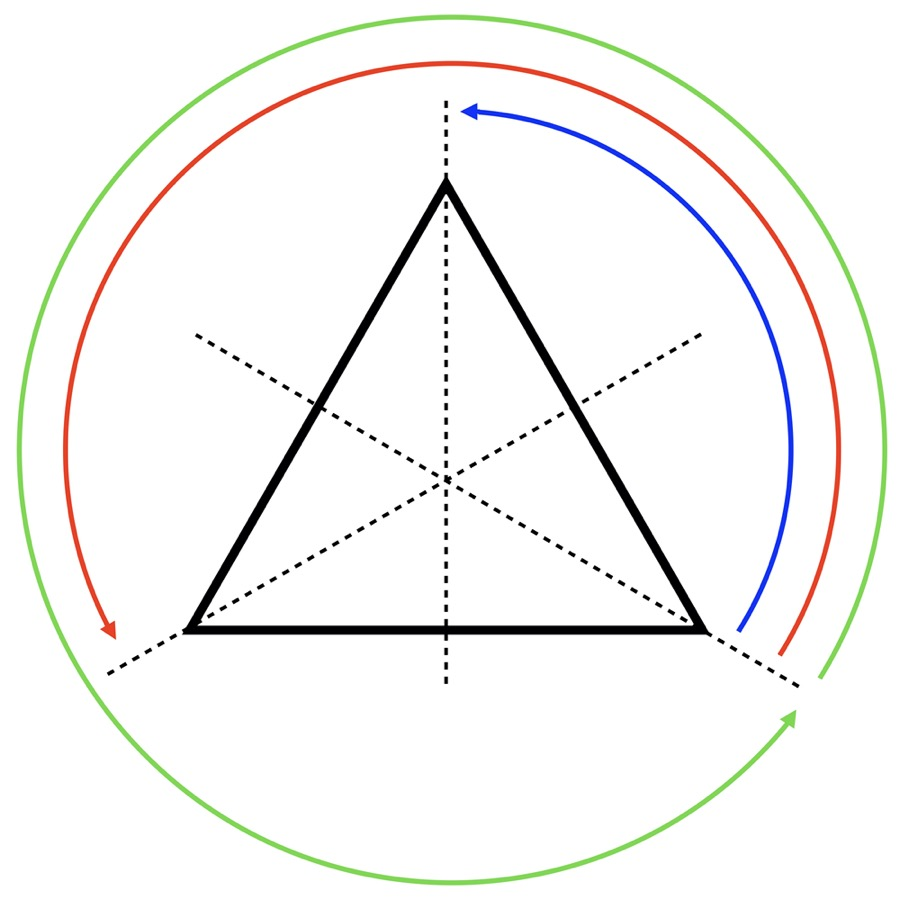
\includegraphics[width=.34\textwidth]{
plane-tessellations-assets/dihedral-triangle
}
\end{center}

\noindent
The rotation by $120^\circ$ and one reflection
generate this group. The thesis records this
in a \emph{Cayley graph}: for a group $G$ with
a generating set $S$, the vertices are the
elements of $G$, and there is an arrow from
$a$ to $b$, coloured by $s\in S$, whenever
$as=b$. Cayley graphs of symmetry groups of
periodic tilings are again tilings of the
plane; see \cite{CoxeterMoser1957}.

\begin{definition}
\label{definition-rosette}
The \emph{dihedral group} $d_n$, $n\geq3$, is
the symmetry group of a regular $n$-gon. It
consists of $n$ rotations and $n$ reflections.
The \emph{cyclic group} $c_n$ is its subgroup
of $n$ rotations. For $n=1,2$: $c_1$ is
trivial, $d_1$ is generated by one reflection,
$c_2$ by one half-turn, and $d_2$ by two
reflections in perpendicular lines.
\end{definition}

\noindent
The group $c_n$ is the symmetry group of a
regular $n$-gon from which half of each side
has been removed, so that no reflection
survives.

\begin{center}
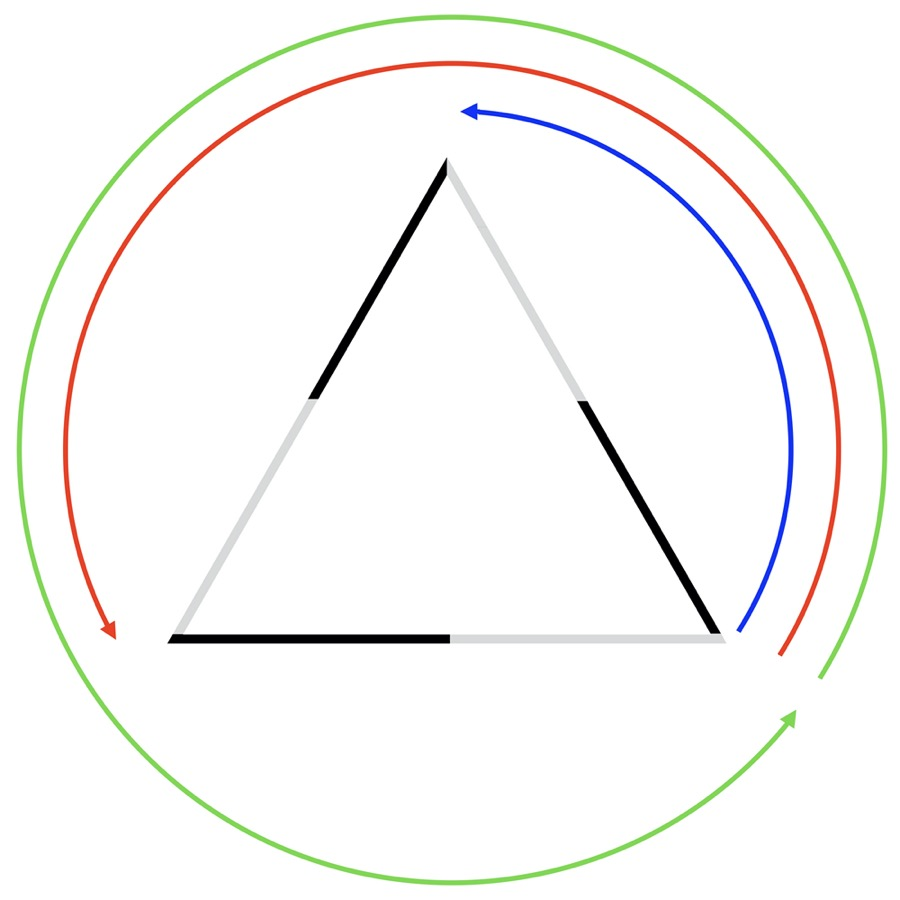
\includegraphics[width=.34\textwidth]{
plane-tessellations-assets/cyclic-triangle
}
\end{center}

\begin{theorem}
\label{theorem-rosette}
If the symmetry group of a tiling contains no
translations, then it is one of the groups
$c_n$ or $d_n$. It is $c_n$ if it consists of
rotations only \cite{GrunbaumShephard1987}.
\end{theorem}

\noindent
These are the \emph{rosette groups} or
\emph{point groups}. None of Escher's periodic
drawings has a rosette group
\cite{Schattschneider2004}.

\section{Frieze groups}
\label{section-frieze}

\noindent
If a symmetry group contains a translation it
contains all its multiples, so it is infinite.
A \emph{frieze} is a pattern whose symmetry
group contains translations, all of them
multiples of a single one. A frieze lives in
a strip, and can be made into a tiling of the
plane by stacking copies of the strip so that
no new translations appear.

\begin{theorem}
\label{theorem-frieze}
There are exactly 7 symmetry groups of
friezes \cite{GrunbaumShephard1987}.
\end{theorem}

\noindent
Their names are
$$
p1,\quad p11g,\quad p1m1,\quad p2,\quad
p2mg,\quad p11m,\quad p2mm.
$$
The letter $p$ stands for primitive cell. The
next symbol is the order of the largest
rotation: $2$ if there are half-turns, $1$ if
there are none. The third symbol is $m$ if
there is a reflection in a line perpendicular
to the translation, and $1$ or nothing
otherwise. The last symbol is $m$ if there is
a reflection in the line of the strip, $g$ if
there is only a glide reflection along it.

The count needs a word of care. The group
$p11g$ is generated by one glide reflection,
whose square is the shortest translation; the
group $p1$ is generated by one translation.
Both are infinite cyclic groups, but the
patterns look different. The same happens for
the rosette groups $d_1$ and $c_2$, both of
order two.

\begin{definition}
\label{definition-same-type}
Two symmetry groups are of the \emph{same
type} if there is an isomorphism between them
that sends rotations to rotations,
translations to translations, reflections to
reflections and glide reflections to glide
reflections.
\end{definition}

\noindent
The seven frieze groups are pairwise of
different type. Cayley graphs alone do not
detect this: isomorphic groups may have very
different Cayley graphs, and one group has
several, for instance the group of the
triangle generated by two reflections, or by
a reflection and a rotation.

\section{Periodic tilings}
\label{section-periodic}

\begin{definition}
\label{definition-periodic}
A tiling is \emph{periodic} if its symmetry
group contains two translations with linearly
independent vectors.
\end{definition}

\noindent
The thesis opens this subject with two of
Escher's drawings, one of horsemen and one of
winged horses. In the second all the figures
look the same way and the symmetry group
consists of translations only; it is the
group $p1$ below. In the first the horsemen
of one colour are mirror images of those of
the other colour. A reflection in a vertical
line does not preserve the drawing, but the
reflection followed by a vertical translation
by half a period does. This symmetry group
consists of translations and glide
reflections; it is the group $pg$ below. The
two groups are not of the same type, and this
is the precise sense in which the two drawings
are different.

\begin{theorem}
\label{theorem-seventeen}
There are exactly 17 symmetry groups of
periodic tilings, up to the equivalence of
Definition \ref{definition-same-type}
\cite{GrunbaumShephard1987}.
\end{theorem}

\noindent
According to \cite{Martin1982}, the result
was first published by Fedorov in 1891 and
found again by Fricke and Klein in 1897 and
by P\'olya and Niggli in 1924.

\section{Preliminaries on isometries}
\label{section-preliminaries}

\noindent
The following facts are used in the
constructions of Section
\ref{section-seventeen}. Proofs are in
\cite{Martin1982}. We write $\sigma_l$ for
the reflection in the line $l$,
$r_{P,\theta}$ for the rotation about $P$ by
the angle $\theta$, counterclockwise, $S_P$
for the half-turn $r_{P,180}$, $t_{AB}$ for
the translation that sends $A$ to $B$, and
$\gamma_l$ for a glide reflection with axis
$l$. A product is read from right to left.

\begin{proposition}
\label{proposition-isometries}
\begin{enumerate}
\item Given congruent triangles
$\triangle PQR$ and $\triangle ABC$, there is
a unique isometry $f$ with $f(P)=A$,
$f(Q)=B$, $f(R)=C$.
\item Every isometry is a product of at most
three reflections.
\item If $l$ and $m$ are parallel, then
$\sigma_m\sigma_l$ is the translation by
twice the vector from $l$ to $m$
perpendicular to both. Every translation
arises in this way.
\item If $l$ and $m$ meet at $P$ and the
directed angle from $l$ to $m$ is $\theta/2$,
then $\sigma_m\sigma_l=r_{P,\theta}$. Every
rotation arises in this way.
\item The product
$\sigma_n\sigma_m\sigma_l$ is a glide
reflection if and only if the lines $l,m,n$
are neither concurrent nor all parallel. If
$m$ and $n$ are perpendicular to $l$, it is
the glide reflection with axis $l$ and
translation vector twice the vector from $m$
to $n$.
\end{enumerate}
\end{proposition}

\begin{definition}
\label{definition-n-centre}
Let $G$ be a group of isometries. A point $P$
is an \emph{$n$-centre} of $G$ if the
rotations in $G$ about $P$ form a cyclic
group of order $n\geq2$.
\end{definition}

\begin{proposition}
\label{proposition-centres}
Every element of $G$ sends $n$-centres of $G$
to $n$-centres of $G$.
\end{proposition}

\begin{theorem}[Crystallographic restriction]
\label{theorem-crystallographic-restriction}
A rotation in the symmetry group of a periodic
tiling has order 2, 3, 4 or 6.
\end{theorem}

\section{Presentations}
\label{section-presentations}

\noindent
Let $S$ be a set. A \emph{word} in $S$ is a
finite product of powers $s^n$ of elements of
$S$, with $n$ an integer. A word is
\emph{reduced} if no two consecutive powers
have the same base and no exponent is zero;
every word can be reduced by replacing
$s^ms^n$ with $s^{m+n}$ and deleting $s^0$.
Reduced words, with concatenation followed by
reduction, form the \emph{free group} $F[S]$.

Given words $r_i$ in $S$, let $R$ be the
smallest normal subgroup of $F[S]$ that
contains all the $r_i$. One writes
$$
G=\langle\, s_j \mid r_i=e \,\rangle
$$
when $G$ is isomorphic to $F[S]/R$, and calls
this a \emph{presentation} of $G$ by
generators and relations. For example, to
make two generators $a$ and $b$ commute one
imposes the relation $b^{-1}a^{-1}ba=e$.

\section{The seventeen groups}
\label{section-seventeen}

\noindent
Let $G$ be the symmetry group of a periodic
tiling. A \emph{unit cell} is a parallelogram
spanned by two shortest independent
translations of $G$; its images under the
translations of $G$ cover the plane. A
\emph{fundamental region} is a region whose
images under all of $G$ cover the plane
without overlapping in their interiors.
Neither is unique. A fundamental region can
be chosen inside a unit cell, and the two
coincide only for the group $p1$.

For each group the thesis shows a periodic
tiling with that group. For 13 groups it is a
drawing by Escher. According to
\cite{Schattschneider2004}, Escher made
drawings for 16 of the 17 groups; those for
$cmm$, $p4m$ and $p6m$ are sketches, and
there is no record of a drawing with group
$pm$. For
these four groups the thesis uses plates of
\cite{Jones1856}.

In the diagrams below the pale parallelogram
is a unit cell $ABCD$ and the darker region is
a fundamental region. The marks are:
\begin{center}
\begin{tabular}{ll}
solid line & axis of a reflection \\
dashed line & axis of a glide reflection \\
lozenge & 2-centre \\
triangle & 3-centre \\
square & 4-centre \\
hexagon & 6-centre
\end{tabular}
\end{center}
Blue marks belong to a generating set of the
group; red marks are other symmetries. The groups are taken in the order
of the largest rotation they contain: 6, 4
and 3, then 2, then none. In each case a
generating set is found geometrically and
then a presentation is given, with $u,v,w,x$
standing for the generators in the order
listed.

\subsection{The group $p6$}
\label{subsection-p6}

This is the only group with rotations of
order 6 and no reflections. Suppose $G$
contains $r_{A,60}$, and let $M$ be a centre
of rotation nearest to $A$. If $M$ were a
centre of order 3, 4 or 6, then writing both
rotations as products of two reflections, one
of them in the line $AM$, one finds that the
product of the two rotations is a rotation
about a point closer to $A$ than $M$. Hence
$M$ is a 2-centre. The product
$S_Mr_{A,60}^{-1}$ is a rotation by
$120^\circ$ about a point $G$, a 3-centre.
The point $B=S_M(A)$ is a 6-centre, and
$t_{AB}=S_MS_A$ is a shortest translation.
With $N=r_{A,60}(M)$ and $C=S_N(A)$ we get
the second shortest translation
$t_{AC}=S_NS_A$.

\begin{center}
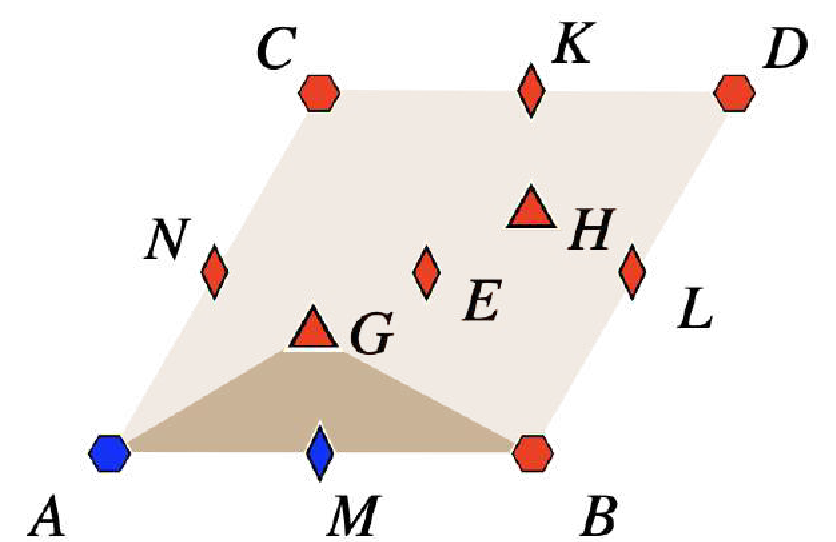
\includegraphics[width=.5\textwidth]{
plane-tessellations-assets/cell-p6
}
\end{center}

\noindent
The triangle $ABG$ is a fundamental region.
Since $S_N=r_{A,60}S_Mr_{A,60}^{-1}$,
$$
p6=\langle t_{AB},t_{AC},r_{A,60}\rangle
=\langle r_{A,60},S_M\rangle ,
$$
$$
p6=\langle u,v\mid
u^6=v^2=(vu^{-1})^3=e\rangle .
$$
The third relation is the order of the
rotation about $G$. The relations for the
other centres in the cell follow, because
those rotations are conjugates of $u$, $v$
and $vu^{-1}$; for example
$(uvu^{-1})^2=uv^2u^{-1}=e$ for $S_N$.

\subsection{The group $p6m$}
\label{subsection-p6m}

Add to $p6$ a reflection. It must send
centres of rotation to centres of rotation of
the same order, and every such choice gives
the same group. Take $\sigma_{CM}$.
Conjugating by the rotations one obtains
reflections in the sides and the diagonals of
the cell and in the lines through the
3-centres, and composing reflections with
half-turns one obtains glide reflections.

\begin{center}
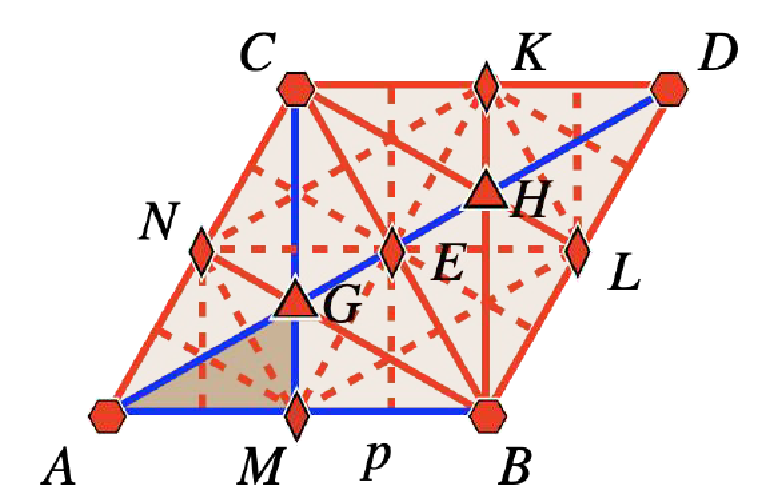
\includegraphics[width=.5\textwidth]{
plane-tessellations-assets/cell-p6m
}
\end{center}

\noindent
The lines $CM$, $AB$ and $AD$ bound a triangle
with angles $90^\circ$ at $M$, $30^\circ$ at
$A$ and $60^\circ$ at $G$, a fundamental
region. Since
$\sigma_{CM}\sigma_{AB}=S_M$ and
$\sigma_{AD}\sigma_{AB}=r_{A,60}$,
$$
p6m=\langle t_{AB},t_{AC},r_{A,60},
\sigma_{CM}\rangle
=\langle\sigma_{CM},\sigma_{AB},
\sigma_{AD}\rangle ,
$$
$$
p6m=\langle u,v,w\mid u^2=v^2=w^2=
(uv)^2=(uw)^3=(wv)^6=e\rangle .
$$

\subsection{The group $p3$}
\label{subsection-p3}

Suppose the rotations of largest order are of
order 3, and there are no reflections. A
3-centre and a 4-centre cannot occur
together, since the product of the two
rotations would be a rotation by $150^\circ$,
against Theorem
\ref{theorem-crystallographic-restriction};
a 3-centre and a 2-centre would produce a
rotation of order 6. So all centres are
3-centres. Let $r_{A,120}\in G$ and let $G$
be a 3-centre nearest to $A$. The translation
$t_{AG}$ is not in the group, since
$r_{G,120}t_{AG}$ would be a rotation about a
point closer to $A$ than $G$. The shortest
translations are $t_{AB}$ and $t_{AC}$ with
$B=r_{G,120}(A)$ and $C=r_{G,-120}(A)$, and
$$
t_{AB}=r_{G,120}\,r_{A,-120},\qquad
t_{AC}=r_{G,-120}\,r_{A,120}.
$$

\begin{center}
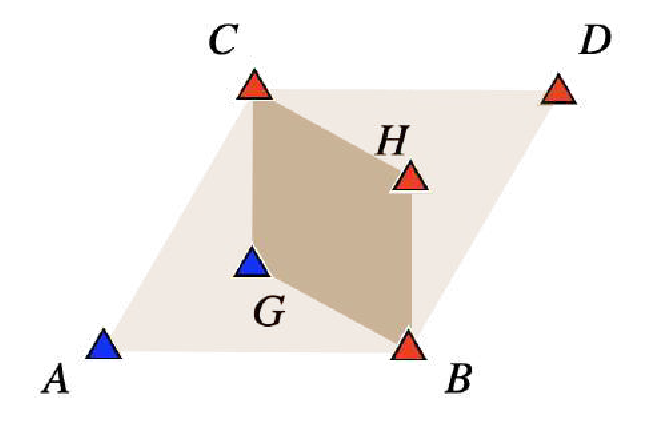
\includegraphics[width=.45\textwidth]{
plane-tessellations-assets/cell-p3
}
\end{center}

\noindent
There are three classes of 3-centres: the
vertices of the cell, and the centres $G$ and
$H$ of the two equilateral triangles into
which a diagonal divides it. Thus
$$
p3=\langle t_{AB},t_{AC},r_{A,120}\rangle
=\langle r_{A,120},r_{G,120}\rangle ,
$$
$$
p3=\langle u,v\mid u^3=v^3=(uv)^3=e\rangle .
$$
The third relation holds because
$r_{A,120}r_{G,120}$ is a rotation by
$240^\circ$, about a 3-centre of the third
class.

\subsection{The group $p31m$}
\label{subsection-p31m}

There are two ways to add a reflection to
$p3$. In the first the axis is the side $AB$
of the cell. Conjugation by the rotations
gives reflections in the other sides and in
the short diagonal $BC$. The axes pass
through the 3-centres at the vertices of the
cell but not through $G$ and $H$.

\begin{center}
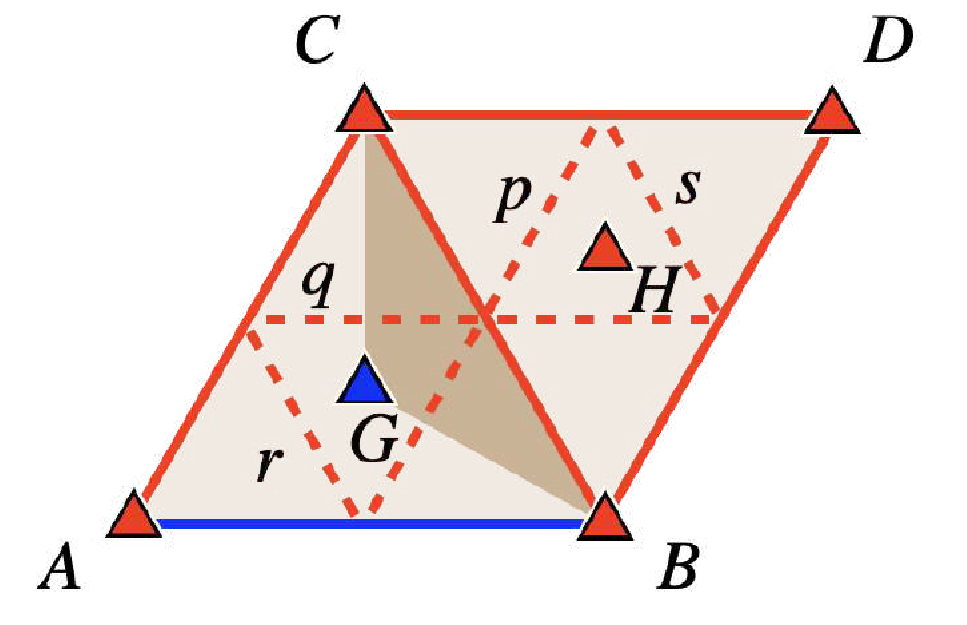
\includegraphics[width=.5\textwidth]{
plane-tessellations-assets/cell-p31m
}
\end{center}

\noindent
Since
$\sigma_{AC}=r_{G,-120}\sigma_{AB}r_{G,120}$
and $r_{A,120}=\sigma_{AC}\sigma_{AB}$,
$$
p31m=\langle t_{AB},t_{AC},r_{A,120},
\sigma_{AB}\rangle
=\langle r_{G,120},\sigma_{AB}\rangle ,
$$
$$
p31m=\langle u,v\mid
u^3=v^2=(u^{-1}vuv)^3=e\rangle .
$$

\subsection{The group $p3m1$}
\label{subsection-p3m1}

In the second way the axis is the long
diagonal $AD$, which passes through all three
kinds of 3-centres. Conjugation gives the
reflections in the lines $BG$, $CG$, $BH$,
$CH$.

\begin{center}
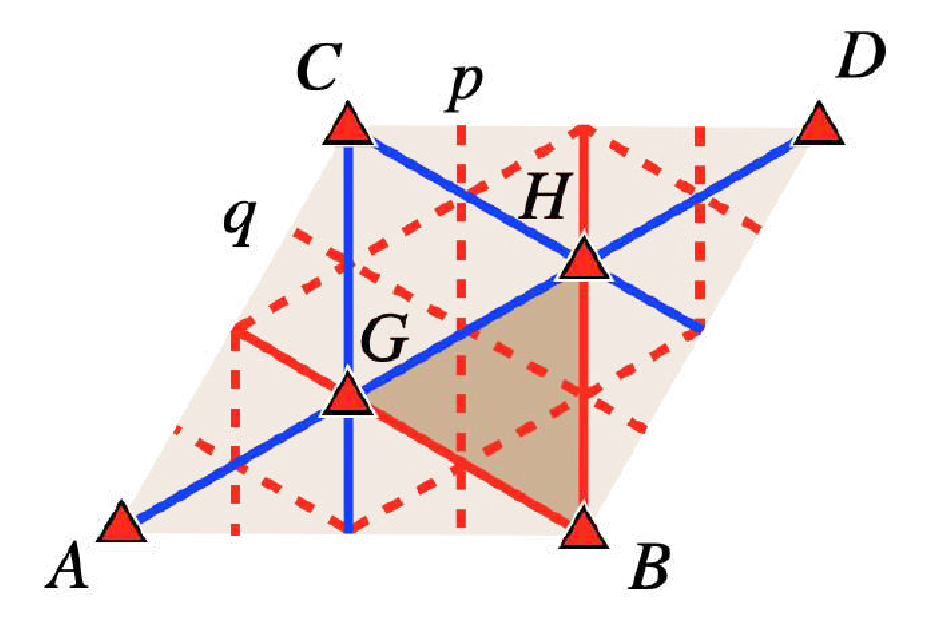
\includegraphics[width=.5\textwidth]{
plane-tessellations-assets/cell-p3m1
}
\end{center}

\noindent
The lines $AD$, $CG$ and $CH$ bound the
equilateral triangle $CGH$, which is also a
fundamental region, and the group is
generated by the reflections in its sides:
$$
p3m1=\langle t_{AB},t_{AC},r_{A,120},
\sigma_{AD}\rangle
=\langle\sigma_{AD},\sigma_{CG},
\sigma_{CH}\rangle ,
$$
$$
p3m1=\langle u,v,w\mid u^2=v^2=w^2=
(uv)^3=(vw)^3=(wu)^3=e\rangle .
$$
None of Escher's drawings with this group is
monohedral.

\subsection{The group $p4$}
\label{subsection-p4}

This is the only group with rotations of
order 4 and no reflections. By Theorem
\ref{theorem-crystallographic-restriction}
only 4-centres and 2-centres occur. Let
$r_{A,90}\in G$ and let $M$ be a centre
nearest to $A$. If $M$ were a 4-centre, then
$r_{M,90}r_{A,90}$ would be a half-turn
about a point closer to $A$, so $M$ is a
2-centre. The product $S_Mr_{A,-90}$ is a
rotation of order 4 about a point $E$, the
4-centre nearest to $A$. The translation
$t_{AE}$ is not in the group. With
$N=r_{A,90}(M)$, $B=S_M(A)$ and $C=S_N(A)$
the shortest translations are
$t_{AB}=S_MS_A$ and $t_{AC}=S_NS_A$; they are
perpendicular and of equal length.

\begin{center}
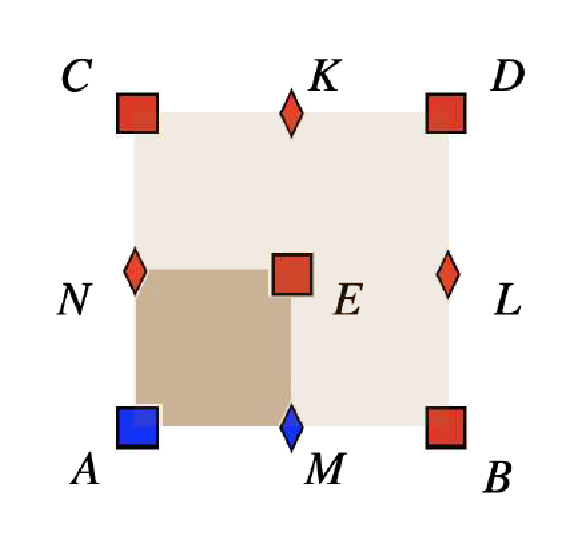
\includegraphics[width=.4\textwidth]{
plane-tessellations-assets/cell-p4
}
\end{center}

$$
p4=\langle t_{AB},t_{AC},r_{A,90}\rangle
=\langle r_{A,90},r_{E,90}\rangle
=\langle r_{A,90},S_M\rangle ,
$$
$$
p4=\langle u,v\mid u^4=v^2=(uv)^4=e\rangle .
$$

\subsection{The group $p4m$}
\label{subsection-p4m}

There are two ways to add a reflection to
$p4$, according to whether the axis passes
through the 4-centres. In the first take
$\sigma_{AE}$. One obtains the reflections in
the sides of the cell, in its two diagonals
and in the two lines through $E$ parallel to
the sides, and four glide reflections.

\begin{center}
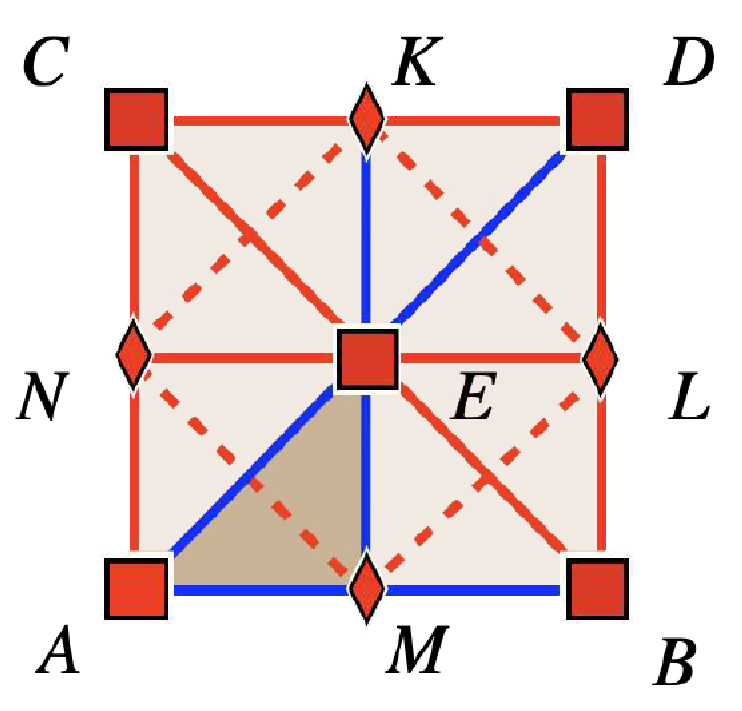
\includegraphics[width=.4\textwidth]{
plane-tessellations-assets/cell-p4m
}
\end{center}

\noindent
The triangle $AME$ is a fundamental region,
with angles $45^\circ$ at $A$ and $E$ and
$90^\circ$ at $M$, and
$$
p4m=\langle t_{AB},t_{AC},r_{A,90},
\sigma_{AE}\rangle
=\langle\sigma_{AE},\sigma_{AB},
\sigma_{ME}\rangle ,
$$
$$
p4m=\langle u,v,w\mid u^2=v^2=w^2=
(uv)^4=(vw)^2=(wu)^4=e\rangle .
$$

\subsection{The group $p4g$}
\label{subsection-p4g}

In the second way the axis avoids the
4-centres. Take $\sigma_{MN}$. Conjugation by
$r_{E,90}$ gives the reflections in the lines
$NK$, $KL$, $LM$, and composition with the
rotations gives glide reflections.

\begin{center}
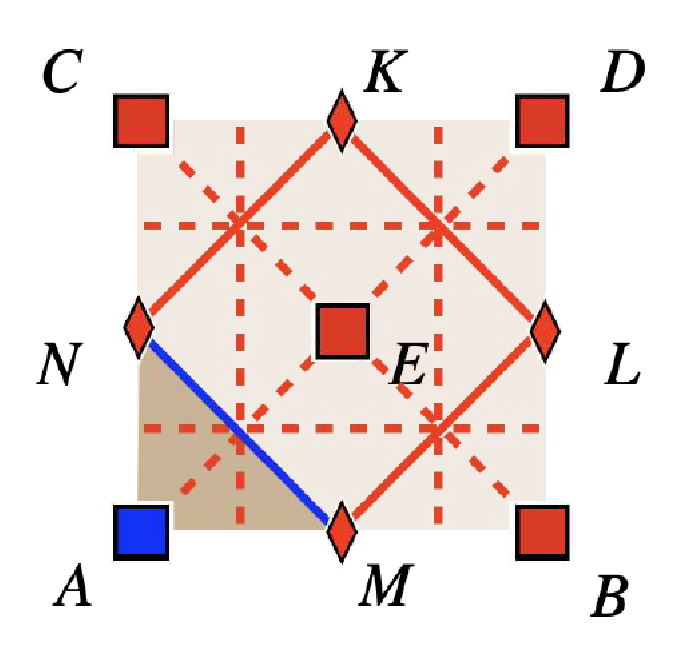
\includegraphics[width=.4\textwidth]{
plane-tessellations-assets/cell-p4g
}
\end{center}

\noindent
Since $r_{E,-90}$ is the conjugate of
$r_{A,90}$ by $\sigma_{MN}$,
$$
p4g=\langle t_{AB},t_{AC},r_{A,90},
\sigma_{MN}\rangle
=\langle r_{A,90},\sigma_{MN}\rangle ,
$$
$$
p4g=\langle u,v\mid
u^4=v^2=(vu^{-1}vu)^2=e\rangle .
$$
The third relation is the order of the
half-turn $S_M$: the line $MN$ and its image
under $r_{A,-90}$ are perpendicular and meet
at $M$.

\subsection{The group $p2$}
\label{subsection-p2}

The rotations are half-turns and there are no
reflections. Let $S_E\in G$ and let $t_{PR}$
and $t_{PQ}$ be shortest independent
translations. Then $S_N=S_Et_{PR}$ and
$S_M=S_Et_{PQ}$ are half-turns, and the
vectors $PR$ and $PQ$ are twice the vectors
$NE$ and $ME$. Conjugating and composing
gives half-turns about the four vertices of a
parallelogram $ABDC$, about the midpoints
$M,N,G,F$ of its sides and about its centre
$E$.

\begin{center}
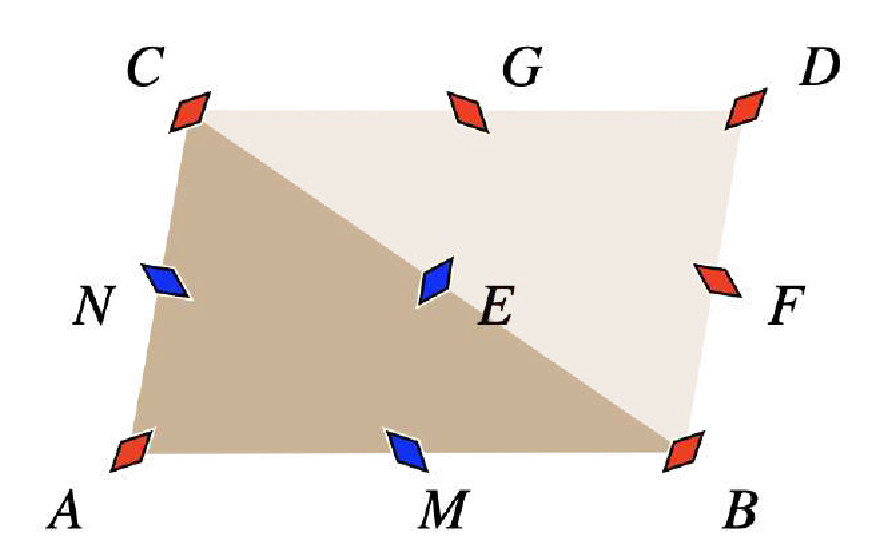
\includegraphics[width=.5\textwidth]{
plane-tessellations-assets/cell-p2
}
\end{center}

$$
p2=\langle t_{AB},t_{AC},S_E\rangle
=\langle S_E,S_M,S_N\rangle ,
$$
$$
p2=\langle u,v,w\mid
u^2=v^2=w^2=(uvw)^2=e\rangle .
$$
The last relation says that the product of
three half-turns is a half-turn.

\subsection{The group $cmm$}
\label{subsection-cmm}

When the symmetry group of a periodic tiling
contains a reflection or a glide reflection,
the unit cell can be taken rectangular or
rhombic. The group $cmm$ arises from $p2$ by
adding a reflection when the cell is
rhombic. The axis must be a diagonal
of the rhombus, say $AE$. Since
$S_E=\sigma_{AE}\sigma_{BE}$, the reflection
in the other diagonal is in the group as
well. There are four glide reflections in the
cell, with axes joining midpoints of adjacent
sides.

\begin{center}
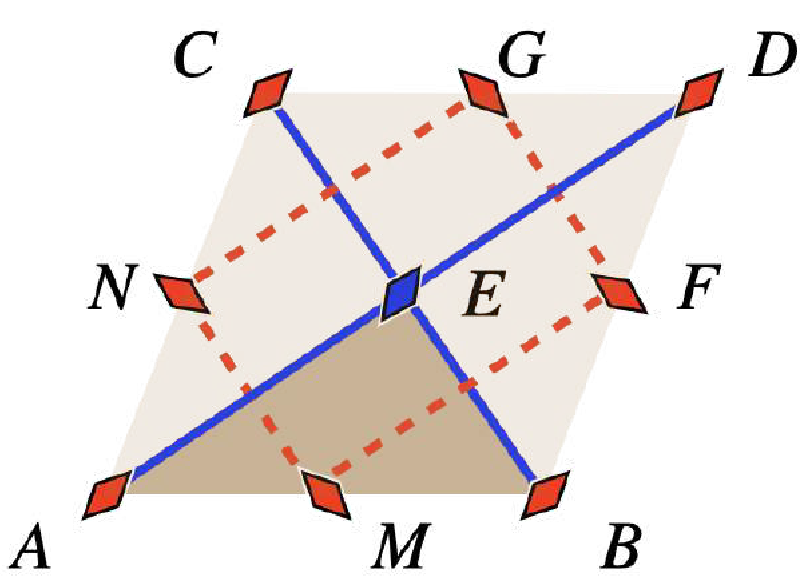
\includegraphics[width=.5\textwidth]{
plane-tessellations-assets/cell-cmm
}
\end{center}

$$
cmm=\langle t_{AB},t_{AC},S_E,\sigma_{AE},
\sigma_{BE}\rangle
=\langle\sigma_{AE},\sigma_{BE},S_M\rangle ,
$$
$$
cmm=\langle u,v,w\mid u^2=v^2=w^2=
(uv)^2=(uwvw)^2=e\rangle .
$$
Here $uv$ is $S_E$ and $uwvw$ is $S_A$.

\subsection{The group $pmm$}
\label{subsection-pmm}

Now the cell is rectangular and the axis of
the added reflection is parallel to a side.
It may pass through 2-centres or not. In the
first case take $\sigma_{AM}$; since
$S_A=\sigma_{AM}\sigma_{AN}$, the reflection
$\sigma_{AN}$ is in the group too. (If the
cell is a square one could also add the
reflection in a diagonal, but then one
arrives at $p4m$.)

\begin{center}
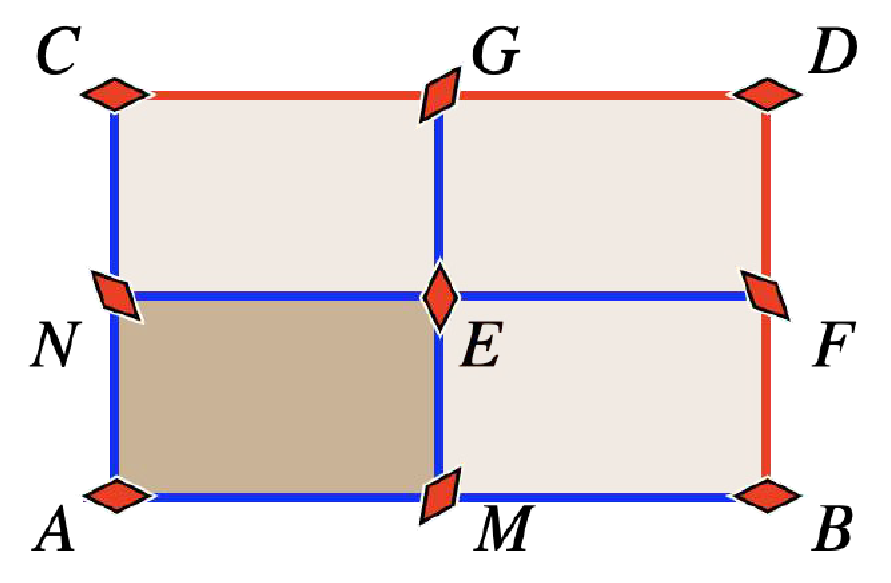
\includegraphics[width=.5\textwidth]{
plane-tessellations-assets/cell-pmm
}
\end{center}

\noindent
The rectangle $AMEN$ is a fundamental region
and the group is generated by the reflections
in its sides:
$$
pmm=\langle t_{AB},t_{AC},S_E,\sigma_{AM},
\sigma_{AN}\rangle
=\langle\sigma_{AN},\sigma_{AM},
\sigma_{ME},\sigma_{NE}\rangle ,
$$
$$
pmm=\langle u,v,w,x\mid u^2=v^2=w^2=x^2=
(uv)^2=(vw)^2=(wx)^2=(xu)^2=e\rangle .
$$

\subsection{The group $pmg$}
\label{subsection-pmg}

In the second case the axis passes halfway
between two rows of 2-centres. Take the
reflection $\sigma_p$ in the perpendicular
bisector $p$ of $AM$. Composing half-turns
with $\sigma_p$ gives glide reflections whose
axes are the lines of 2-centres perpendicular
to $p$.

\begin{center}
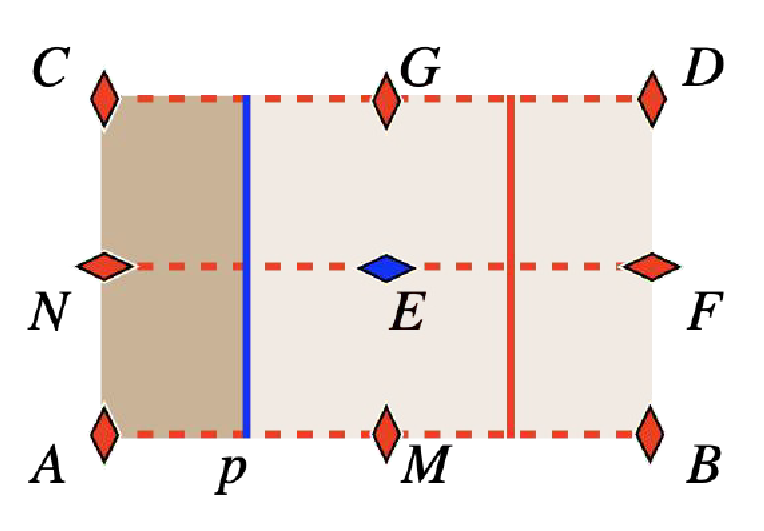
\includegraphics[width=.5\textwidth]{
plane-tessellations-assets/cell-pmg
}
\end{center}

\noindent
Since $S_E=\sigma_pS_N\sigma_p$ and
$S_M=\sigma_pS_A\sigma_p$,
$$
pmg=\langle t_{AB},t_{AC},S_E,
\sigma_p\rangle
=\langle S_N,S_A,\sigma_p\rangle ,
$$
$$
pmg=\langle u,v,w\mid
u^2=v^2=w^2=e,\ uwu=vwv\rangle .
$$
The last relation says that conjugating
$\sigma_p$ by $S_N$ or by $S_A$ gives the same
reflection.

\subsection{The group $pgg$}
\label{subsection-pgg}

The last extension of $p2$ adds a glide
reflection and no reflection. If the axis
passed through a 2-centre, the product of the
half-turn and the glide reflection would be a
reflection, and one would arrive at $pmg$. So
the cell is rectangular and the axis $p$
passes halfway between two rows of 2-centres;
take the perpendicular bisector of $AM$. The
translation vector of $\gamma_p$ must be $AN$:
the only 2-centre to which $\gamma_p$ can send
$M$ is $N$, since otherwise composing with a
translation would give a reflection. Then
$\gamma_q=\gamma_pS_A$ is a glide reflection
whose axis $q$ is the perpendicular bisector
of $AN$, with translation vector $AM$.

\begin{center}
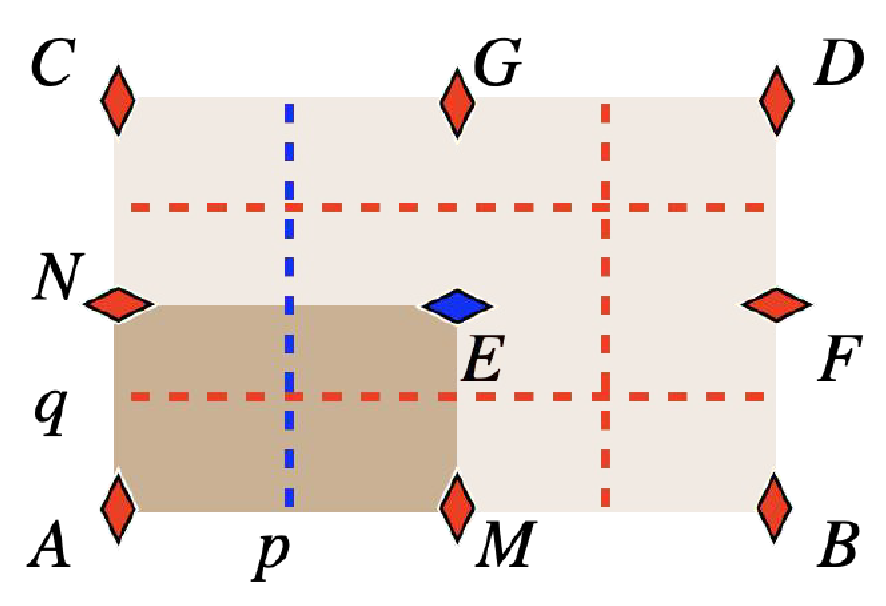
\includegraphics[width=.5\textwidth]{
plane-tessellations-assets/cell-pgg
}
\end{center}

\noindent
Since $\gamma_p^2=t_{AC}$ and
$\gamma_q^2=t_{AB}$,
$$
pgg=\langle t_{AB},t_{AC},S_E,
\gamma_p\rangle
=\langle\gamma_p,\gamma_q\rangle ,
$$
$$
pgg=\langle u,v\mid
(uv)^2=(u^{-1}v)^2=e\rangle .
$$
The two relations are the orders of two
half-turns.

\subsection{The group $p1$}
\label{subsection-p1}

The simplest group has no rotations,
reflections or glide reflections. It is
generated by two translations with linearly
independent vectors. The unit cell is any
parallelogram and is also a fundamental
region.

\begin{center}
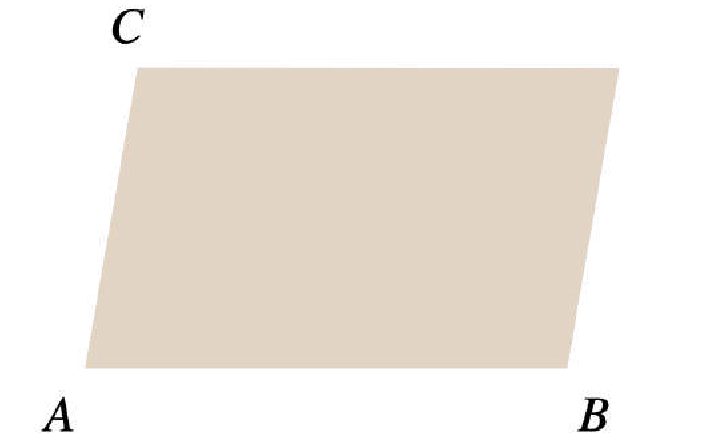
\includegraphics[width=.4\textwidth]{
plane-tessellations-assets/cell-p1
}
\end{center}

$$
p1=\langle t_{AB},t_{AC}\rangle
=\langle u,v\mid uv=vu\rangle .
$$

\subsection{The group $cm$}
\label{subsection-cm}

Add a reflection to $p1$ so that the cell is
rhombic. The axis is a
diagonal of the cell, say $AD$. Then
$\gamma_p=\sigma_{AD}t_{AB}$ is a glide
reflection whose axis $p$ is parallel to $AD$
and passes through the midpoints of $AC$ and
$CD$, with translation vector
$\frac{1}{2}AD$; similarly
$\gamma_q=\sigma_{AD}t_{AC}$.

\begin{center}
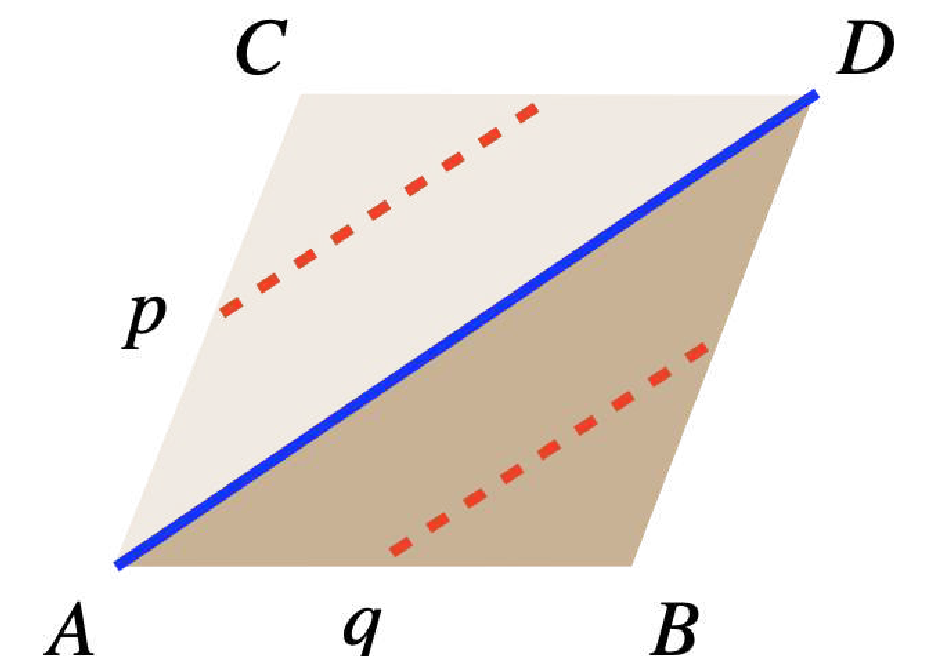
\includegraphics[width=.5\textwidth]{
plane-tessellations-assets/cell-cm
}
\end{center}

\noindent
Since $\gamma_p^2=t_{AD}$ and
$t_{AD}t_{AB}^{-1}=t_{AC}$,
$$
cm=\langle t_{AB},t_{AC},\sigma_{AD}\rangle
=\langle\sigma_{AD},\gamma_p\rangle ,
$$
$$
cm=\langle u,v\mid u^2=e,\ uv^2=v^2u\rangle .
$$
The second relation says that $\sigma_{AD}$
commutes with $t_{AD}$, whose vector is
parallel to the axis.

\subsection{The group $pm$}
\label{subsection-pm}

Add a reflection to $p1$ so that the cell is
rectangular. The axis is parallel to a side;
take $\sigma_{AC}$. Conjugating by $t_{AB}$
gives $\sigma_{BD}$, and
$\sigma_{AC}t_{AB}^{-1}$ is the reflection
$\sigma_{MG}$ in the line halfway between.

\begin{center}
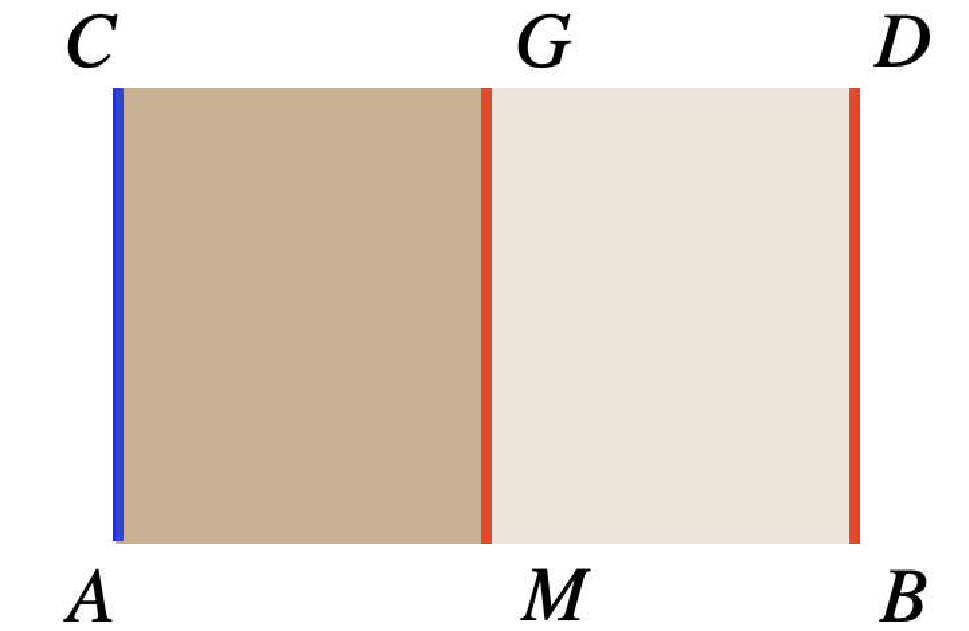
\includegraphics[width=.5\textwidth]{
plane-tessellations-assets/cell-pm
}
\end{center}

$$
pm=\langle t_{AB},t_{AC},\sigma_{AC}\rangle
=\langle t_{AC},\sigma_{AC},
\sigma_{MG}\rangle ,
$$
$$
pm=\langle u,v,w\mid
v^2=w^2=e,\ uv=vu,\ uw=wu\rangle .
$$
The last two relations say that the two
reflections commute with the translation
$t_{AC}$ along their axes.

\subsection{The group $pg$}
\label{subsection-pg}

There is only one way to extend $p1$ by glide
reflections alone. Two glide reflections with
non-parallel axes would produce a rotation,
so all axes are parallel, and the cell can be
taken rectangular with the axes parallel to a
side. The square of a glide reflection is a
translation; take $\gamma_{AM}$ with axis the
line $AB$ and translation vector $AM$, where
$M$ is the midpoint of $AB$. Conjugating by
$t_{AC}$ gives a glide reflection with axis
$CD$, and $\gamma_p=t_{AC}\gamma_{AM}$ is a
glide reflection whose axis $p$ is the line
halfway between $AB$ and $CD$.

\begin{center}
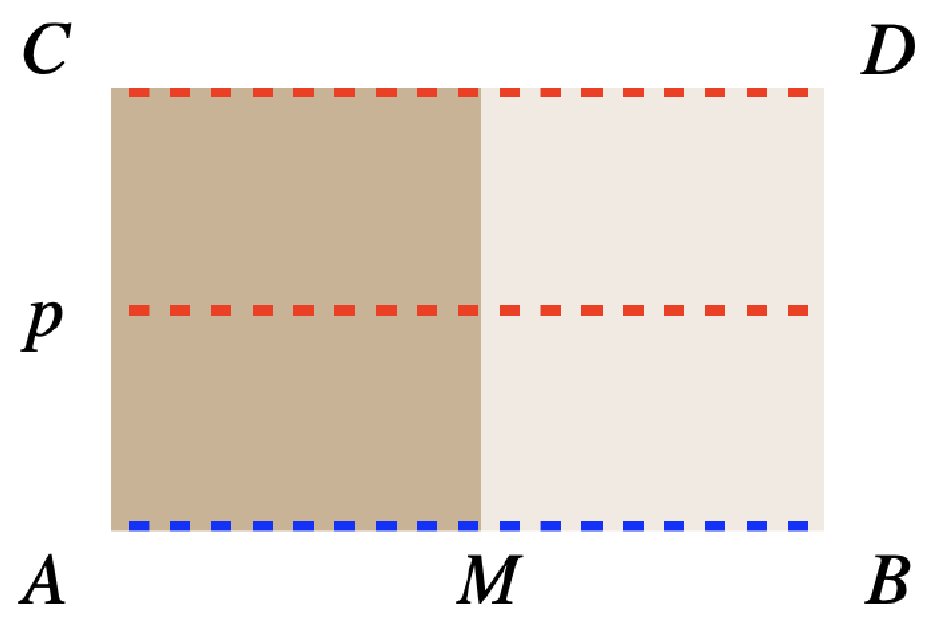
\includegraphics[width=.5\textwidth]{
plane-tessellations-assets/cell-pg
}
\end{center}

$$
pg=\langle t_{AB},t_{AC},
\gamma_{AM}\rangle
=\langle\gamma_{AM},\gamma_p\rangle ,
$$
$$
pg=\langle u,v\mid u^2=v^2\rangle .
$$
Both squares are equal to $t_{AB}$.


\bibliography{my}
\bibliographystyle{amsalpha}

\end{document}
